% Proposal version of the node throughput test, GCS template layout (V2.1-2026JAN12, as ANTRAG_SUPERMUC/common/preamble.tex).
% Built by prelim.sh from results.csv; numbers come from antrag_data.tex (make_antrag.py).
\documentclass[11pt]{article}
\usepackage{times,graphicx,float,amsmath,ifthen,tabularx,enumitem}
\usepackage[usenames,dvipsnames]{xcolor}
\usepackage[T1]{fontenc}
\usepackage{scrlayer-scrpage}
\usepackage{caption}
\usepackage{pgfplots}\pgfplotsset{compat=1.18}
\pgfplotsset{every axis/.append style={font=\small, grid=major, grid style={gray!25}},
  every axis legend/.append style={font=\footnotesize, draw=none, fill=white, fill opacity=0.8, text opacity=1}}
\captionsetup{font=small,labelfont=bf}
\pagestyle{scrheadings}\clearpairofpagestyles
\textwidth 16cm \textheight 23cm
\setlength{\oddsidemargin}{0.1cm}\setlength{\topmargin}{1cm}
\setlength{\headheight}{0cm}\setlength{\headsep}{0cm}\setlength{\footskip}{0.75cm}
\setlength{\parindent}{0cm}\setlength{\parskip}{0.6ex}
\cfoot{\pagemark}\ofoot{\tiny V2.1-2026JAN12}
\setlist{nosep,leftmargin=1.5em}
\newcommand{\gcssection}[1]{\section*{#1}\vspace{-1.5ex}\noindent\rule{\textwidth}{0.4pt}\par}

\newcommand{\DataState}{prelim, 2026-11-27 12:17}
\newcommand{\DataNote}{\textbf{Preliminary.} 10 finished runs (of 25 planned), 4 jobs still queued or running at 2026-11-27 12:17.}

\newcommand{\Lmax}{--}
\newcommand{\FacIntel}{--}
\newcommand{\FacBase}{--}
\newcommand{\Eratio}{--}
\newcommand{\FacList}{}
\newcommand{\StarNote}{$^*$\,best of the configurations finished so far; no speedup given.}
\newcommand{\Complete}{no}
\newcommand{\AntragTable}{%
\begin{tabular}{rlllrrr}
$L$ & node & code & configuration & work units / node-h & speedup & kJ / unit\\
\hline
16 & CPU & ALF CPU & \multicolumn{4}{l}{\emph{running}}\\
16 & GPU & ALF GPU & 4 proc./tile, 3 thr. & 25\,602 & -- & 0.436\\
16 & GPU & ALF GPU Intel-opt. & \multicolumn{4}{l}{\emph{running}}\\
\hline
24 & CPU & ALF CPU & \multicolumn{4}{l}{\emph{running}}\\
24 & GPU & ALF GPU & 4 proc./tile, 3 thr. & 4\,679 & -- & 2.385\\
24 & GPU & ALF GPU Intel-opt. & \multicolumn{4}{l}{\emph{running}}\\
\hline
32 & CPU & ALF CPU & \multicolumn{4}{l}{\emph{running}}\\
32 & GPU & ALF GPU & 2 proc./tile, 7 thr. & 1\,431 & -- & 7.799\\
32 & GPU & ALF GPU Intel-opt. & 4 proc./tile, 1 thr. & 3\,652 & -- & 3.056\\
\hline
36 & CPU & ALF CPU & \multicolumn{4}{l}{\emph{running}}\\
36 & GPU & ALF GPU & 2 proc./tile, 7 thr. & 814 & -- & 13.710\\
36 & GPU & ALF GPU Intel-opt. & \multicolumn{4}{l}{\emph{running}}\\
\end{tabular}}

\begin{document}

\gcssection{Code performance: ALF on SuperMUC-NG Phase 2 (production temperature, $\beta=L$)}
\ifthenelse{\equal{\Complete}{yes}}{}{\textcolor{red}{\small\textbf{Preliminary} -- not all runs finished (\DataState).}\par}

\subsection*{Codes}
\begin{itemize}
\item \textbf{ALF CPU}: ALF (Algorithms for Lattice Fermions), MPI + OpenMP version for CPUs.
\item \textbf{ALF GPU}: our GPU port of ALF (OpenMP offload, oneMKL); thoroughly tested.
\item \textbf{ALF GPU Intel-optimised}: additional optimisations for Intel GPUs (device-side QR decompositions, fused
  kernels, asynchronous updates). Its results cannot be bit-identical to the CPU code (floating-point operations run in a different order on the GPU), so the stochastic process has to be
  validated with long runs; for this LRZ granted a special allocation of 25\,000 GPU-h to project pn93la in November 2026.
  The speedups measured here show that this testing effort pays off.
\end{itemize}
Toolchain: Intel oneAPI 2025.3, Intel MPI 2021.15, oneMKL 2025.3.

\subsection*{Benchmark}
\begin{itemize}
\item Dense complex matrices of dimension $N=L^2$ (256 to 1296), $10L$ per configuration (160 to 360); cost per sweep $\propto N^3$
  (matrix products, QR and LU decompositions).
\item Work unit: one sweep of one independent simulation (one simulation per MPI process).
\item One full node per run, best configuration per node type: CPU node = 112 cores (2 $\times$ Xeon 8480L),
  GPU node = 4 $\times$ Intel Max 1550 (8 tiles).
\item 2 to 5 sweeps timed individually per run; sweep-to-sweep variation $<1\,\%$.
\item CPU node at $L=36$: 112 MPI processes $\times$ 1 thread exceed the node memory (run killed), so 56 $\times$ 2 is the best possible configuration there.
\end{itemize}

\begin{table}[H]
\caption{Throughput of one SuperMUC-NG Phase 2 node at LRZ in its best configuration; speedup relative to the CPU node.
Energy per work unit estimated from vendor ratings (CPU node 700\,W, GPU node 3100\,W). \StarNote}
\label{tab:node}
\begin{center}\setlength{\tabcolsep}{7pt}\renewcommand{\arraystretch}{1.15}\small
\AntragTable
\end{center}
\end{table}

\begin{figure}[H]\centering
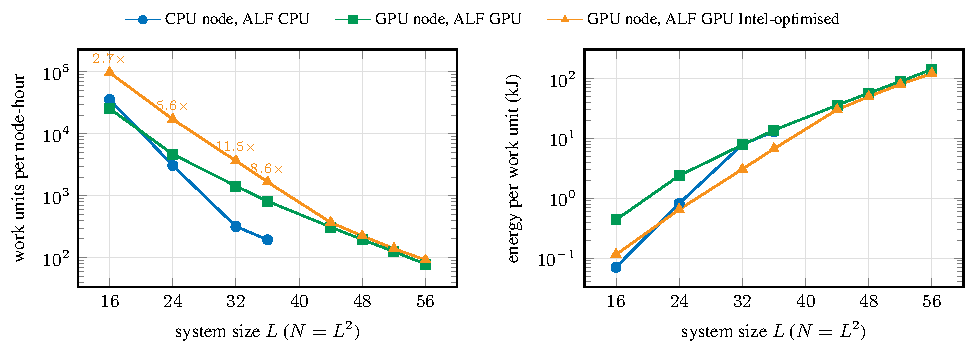
\includegraphics[width=\textwidth]{figures/node_performance}
\caption{Left: node throughput of the best configuration; numbers = speedup of the GPU node (ALF GPU Intel-optimised) over the
CPU node. Right: estimated energy per work unit (vendor power ratings: CPU node 700\,W, GPU node 3100\,W).}
\end{figure}

\subsection*{Result}
\ifthenelse{\equal{\Lmax}{--}}{Results follow when the runs for at least one system size are complete.}{%
\begin{itemize}
\item At $L=\Lmax$ one GPU node gives \textbf{\FacIntel$\times$} the throughput of the CPU node (ALF GPU Intel-optimised;
  \FacBase$\times$ with ALF GPU) at \Eratio$\times$ lower energy per work unit.
\item Speedup of the GPU node (Intel-optimised) over the CPU node: \FacList.
\end{itemize}}
\end{document}
